\documentclass[12pt]{article}
\usepackage[svgnames,x11names,table]{xcolor}
\usepackage{hyperref}
\usepackage{graphicx}
\usepackage{parskip}
\usepackage{float}
\usepackage{amsmath}
\usepackage{amssymb}
\usepackage{enumitem}
\usepackage[thicklines]{cancel}

\hypersetup{
    colorlinks,
    citecolor=black,
    filecolor=black,
    linkcolor=RoyalBlue4,
    urlcolor=RoyalBlue4,
}

\title{PEU 323 Assignment 2}
\author{Mohamed Hussien El-Deeb (201900052)}
\date{}

\begin{document}

\maketitle
\tableofcontents

\section{Problem 1}

\subsection{Problem}

Consider a particle which is free to be anywhere, with equal probability, on a line segment of length $L$.

\renewcommand{\labelenumi}{(\alph{enumi})}
\begin{enumerate}
    \item Find the normalized probability distribution for such a particle.
    \item Calculate $\langle x\rangle $ and $\sigma_{x}$.
    \item Calculate the probability of finding the particle within $\sigma_{x}$ of $\langle x\rangle $.
    \item What are the dimensions of the probability density?
\end{enumerate}

\subsection{Solution}

\begin{enumerate}
    \item $\frac{1}{L} $
    \item \begin{align*}
              \langle x\rangle      & = \frac{1}{L} \int_{0}^{L} x\,dx = \frac{L}{2}               \\
              \sigma_{x}            & = \sqrt{\langle x^2 \rangle - {\langle x \rangle}^2}         \\
              \langle x^2 \rangle   & = \frac{1}{L} \int_{0}^{L} x^2\,dx = \frac{L^2}{3}           \\
              {\langle x \rangle}^2 & = \frac{L^2}{4}                                              \\
              \sigma_{x}            & = \sqrt{\frac{L^2}{3} - \frac{L^2}{4}} = \frac{L}{2\sqrt{3}}
          \end{align*}
    \item $\frac{1}{L} \int_{\frac{L}{2} (1 - \frac{1}{\sqrt{3}})}^{\frac{L}{2} (1 + \frac{1}{\sqrt{3}})}dx = \frac{1}{\sqrt{3}}$
    \item $length^{-1}$
\end{enumerate}

\newpage

\section{Problem 2}

\subsection{Problem}

Buffon's Needle: A needle of length $l$ is dropped at random on a sheet of paper with parallel lines a distance $l$ apart. What is the probability that it crosses a line?

\subsection{Solution}

\begin{figure}[H]
    \centering
    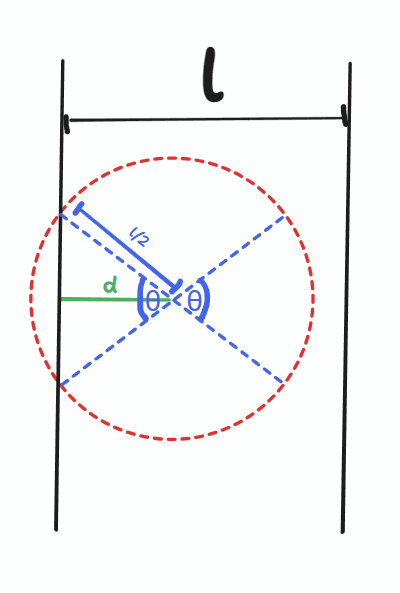
\includegraphics[scale=0.7]{Q2.png}
    \caption{The black lines are the parallel lines of the paper, the red circle represents the possible area covered by the needle on a specific distance d from one of the lines. $\theta$ is the angle in which the needle crosses one of the lines}
\end{figure}

\[
    \cos{\left(\frac{\theta}{2}\right)} = \frac{2d}{l}
\]


\[
    \theta = 2\cos^{-1}{\left(\frac{2d}{l}\right)}
\]


\[
    P(d) = 4\frac{\theta}{2\pi} = \frac{2}{\pi}\cos^{-1}{\left(\frac{2d}{l}\right)}
\]

\[
    P = \int^{\frac{L}{2}}_{0}P(d)\,dd
\]

\[
    = \frac{2}{\pi}\int^{\frac{L}{2}}_{0}\cos^{-1}{\left(\frac{2d}{l}\right)}\,dd
\]

\[
    \because \int{\cos^{-1}{(x)}\,dx} = x \cos^{-1}{(x)}-\sqrt{1-x^2} + c
\]

\[
    \therefore P = \left[\frac{2d}{l} \cos^{-1}{(\frac{2d}{l})}-\sqrt{1-{\left(\frac{2d}{l}\right)}^2}\right]^\frac{L}{2}_0 = \frac{2}{\pi}
\]

\newpage

\section{Problem 3}

\subsection{Problem}

Find the probability distribution for the momentum of a harmonic oscillator with angular frequency $\omega $.

\subsection{Solution}

\[
    y(t) = A \sin (\omega t)
\]

\[
    p = y'(t) = A \omega \cos (\omega t)
\]

\[
    t = \frac{\cos^{-1}(\frac{p}{A\omega})}{\omega}
\]

\[
    p' = - A \omega^2 \sin (\omega t) = - A \omega^2 \sin (\cos^{-1}(\frac{p}{A\omega}))
\]

\[
    p_f = \frac{p}{Aw}
\]

We will absorb all constants and proportionality constants into \(\alpha\)
\[
    \rho(p_f) \propto \frac{1}{p'} = \alpha \csc (\cos^{-1}(p_f))
\]

\[
    \int^1_{-1} \rho(p_f)\,dp_f = \alpha \int^1_{-1}\csc (\cos^{-1}(p_f))\,dp_f = \frac{\pi}{2}
\]

\newpage

\section{Problem 4}

\subsection{Problem}

Consider the probability density for the location of the electron inside the Hydrogen atom:

\begin{equation}
    \rho(r)=A e^{-2 r / a_{0}},
\end{equation}

where $a_{0}$ is the Bohr radius.

\renewcommand{\labelenumi}{(\alph{enumi})}
\begin{enumerate}
    \item Find $A$ which normalizes this probability distribution.

          \textit{Hint:}

          \begin{equation}
              \int_{0}^{\infty} e^{-x} x^{n} d x=n!.
          \end{equation}
    \item Calculate the probability for the electron to be found in a sphere, centered about the origin, of radius $b_{0}$, with $b_{0}<<a_{0}$.

          \textit{P.S.:} You can do this calculation exactly or approximately. The approximate one is much easier.
\end{enumerate}

\subsection{Solution}


\renewcommand{\labelenumi}{(\alph{enumi})}
\begin{enumerate}
    \item
          \[
              \rho(r) = A e^{-2 r / a_{0}}
          \]
          \[
              \rho = \int_{0}^{\infty}{\rho(r)}\,dr = 1
          \]
          \[
              \rho = A \int_{0}^{\infty}{e^{-\frac{2r}{a_{0}}}}\,dr
          \]
          \[
              \because \int{e^{-\alpha x}}\,dx = -\frac{e^{-\alpha x}}{\alpha} + c
          \]
          \[
              \therefore 1 = - \frac{A}{\alpha}{\left[e^{- \alpha r}\right]}^{\infty}_0 = \frac{A}{\alpha}
          \]
          \[
              A = \frac{2}{a_0}
          \]
    \item
          \[
              \rho(r) = \frac{2}{a_0} e^{-2 r / a_{0}}
          \]
          \[
              \frac{2}{a_0}\int_0^{b_0}{e^{-\alpha x}}\,dx = -\frac{2}{\alpha a_0}\left[e^{-\alpha x}\right]^{b_0}_0
          \]
          \[
              = 1 - e^{-2 \frac{b_0}{a_0}} \approx 2 \frac{b_0}{a_0}
          \]
\end{enumerate}

\section{Problem 5}

\subsection{Problem}

Consider the map

\begin{equation}
    f: \mathbb{C} \rightarrow \mathbb{R}_{2 \times 2}
\end{equation}

\[
    x + iy \mapsto
    \begin{pmatrix}
        x & -y \\
        y & x
    \end{pmatrix}
\]

from the complex numbers to the set of $2 \times 2$ real matrices.

\renewcommand{\labelenumi}{(\alph{enumi})}
\begin{enumerate}
    \item Show that this map is an isomorphism. That is, show that it is invertible and that for $z_{1}, z_{2} \in \mathbb{C}$,

          \begin{equation}
              f\left(z_{1} z_{2}\right)=f\left(z_{1}\right) f\left(z_{2}\right)
          \end{equation}

          and hence prove that, in two dimensions, rotations commute.
    \item Prove De Moivre's formula for complex numbers:
          \begin{equation}
              {(r(\cos (\theta)+i \sin (\theta)))}^{n}=r^{n}(\cos (n \theta)+i \sin (n \theta))
          \end{equation}

          and hence prove that

          \begin{equation}
              {\left(\begin{array}{cc}
                          \cos (\theta) & -\sin (\theta) \\
                          \sin (\theta) & \cos (\theta)
                      \end{array}\right)}^{n}=\left(\begin{array}{cc}
                      \cos (n \theta) & -\sin (n \theta) \\
                      \sin (n \theta) & \cos (n \theta)
                  \end{array}\right)
          \end{equation}
\end{enumerate}

\subsection{Solution}

\begin{enumerate}
    \item
          \[
              f\left(z_{1} z_{2}\right) = f((x_1 + iy_1)(x_2 + iy_2)) = f((x_1x_2 - y_1y_2) + i(x_1y_2 + y_1x_2))
          \]
          \[
              =\begin{pmatrix}
                  x_1x_2 - y_1y_2 & -x_1y_2 - y_1x_2 \\
                  x_1y_2 + y_1x_2 & x_1x_2 - y_1y_2  \\
              \end{pmatrix}
          \]
          \[
              f\left(z_{1}\right) f\left(z_{2}\right) = \begin{pmatrix}
                  x_1 & -y_1 \\
                  y_1 & x_1  \\
              \end{pmatrix}\begin{pmatrix}
                  x_2 & -y_2 \\
                  y_2 & x_2  \\
              \end{pmatrix}
          \]
          \[
              = \begin{pmatrix}
                  x_1x_2 - y_1y_2 & -x_1y_2 - y_1x_2 \\
                  x_1y_2 + y_1x_2 & x_1x_2 - y_1y_2  \\
              \end{pmatrix}
          \]

          We can that \(f\left(z_{1} z_{2}\right)\) is just a multiplication of two complex number and that commutes.
    \item \[
              e^{i\theta} = \cos(\theta) + i\sin(\theta)
          \]
          \begin{equation}
              {(r(\cos (\theta)+i \sin (\theta)))}^{n}=r^{n}{(\cos (\theta) + i \sin (\theta))}^n
          \end{equation}
          \[
              =r^{n}e^{in\theta} =  r^{n}(\cos(n\theta) + i\sin(n\theta))
          \]

          Since the rotation transformation is isomorphic.

          \[
              \therefore \left(\begin{array}{cc}
                  \cos (\theta) & -\sin (\theta) \\
                  \sin (\theta) & \cos (\theta)
              \end{array}\right)^{n} \mapsto {(\cos(\theta) + i\sin(\theta))}^n = \cos(n\theta) + i\sin(n\theta)
          \]

          \[
              \mapsto \left(\begin{array}{cc}
                      \cos (n \theta) & -\sin (n \theta) \\
                      \sin (n \theta) & \cos (n \theta)
                  \end{array}\right)
          \]

\end{enumerate}

\newpage

\bibliographystyle{plain}
\bibliography{references}
\nocite{El-Deeb_PEU-323_Assignments}

\end{document}